\section{Appendix}

\subsection{Stan Code} % =================
\begin{verbatim}
data {                             
  int<lower=0> N;                 // N observations
  int<lower=0> p;                 // p predictors
  matrix[N,p] Q;                  // QR decomp - Q
  matrix[p,p] R;                  // QR decomp - R
  int<lower=0, upper=1> hit[N];   // 0/1 outcomes; array of integers
  vector[2] px_pz[N];             // N-dim array of 2-dim vectors
  vector[p] theta_SDs;            // theta prior SDs
}
transformed data{
  matrix[p,p] R_inv;
  R_inv = inverse(R);
}
parameters {                
  real<lower=0> l;                  // length-scale parameter
  real<lower = 0> sigma;            // scale parameter
  real beta0;                       // intercept 
  vector[p] theta;
  vector[N] Z;                      // location random effect
}
transformed parameters {
      vector[p] beta;
      beta = R_inv*theta;
}
model {  
  matrix[N, N] Sigma;
  matrix[N, N] L;                     // Lwr triangular Cholesky decomp
  vector[N] Z_mod;
      
      l ~ lognormal(-2,1);            // E[l] = 0.223
      sigma ~ lognormal(-1.5, 1.5);   // E[sigma] = 0.687
      beta0 ~ normal(0,5);
      
      theta[1] ~ normal(0, theta_SDs[1]);
      theta[2] ~ normal(0, theta_SDs[2]);
      theta[3] ~ normal(0, theta_SDs[3]);
      theta[4] ~ normal(0, theta_SDs[4]);
      theta[5] ~ normal(0, theta_SDs[5]);
      theta[6] ~ normal(0, theta_SDs[6]);
      
      Sigma = cov_exp_quad(px_pz, sigma, l); 
      for (n in 1:N)
        Sigma[n, n] = Sigma[n, n] + 1e-6;
      L = cholesky_decompose(Sigma); // Sigma = LL' 
      
      Z ~ normal(0, 1);  // Each element is N(0,1)
      Z_mod = L * Z; // (Cov matrix Cholesky)*MVN(0,1)
      
      hit ~ bernoulli_logit(beta0 + Q*theta + Z_mod);
}
\end{verbatim}

\subsection{Kriging} % =================

From: ``Statistical Methods for Spatial Data Analysis'' \citep{Schabenberger2004}

The mean is known---Simple Kriging
\begin{enumerate}
\item Spatial data: $\mathbf{Z(s)} = [Z(s_{1}), Z(s_{2}),\hdots, Z(s_{n})]'$

\item Assume: $\mathbf{Z(s) = \mu(s) + e(s)}$, $\mathbf{e(s) \sim (0, \Sigma)}$, where $\mathbf{0, \Sigma}$ known.

\item Goal: find predictor $p(\mathbf{Z};s_{0})$, of $Z(s_{0})$, that minimizes $E\left[ \left(p(\mathbf{Z};s_{0}) - Z(s_{0}) \right)^{2}\right]$ 

\item Consider only linear predictors of the form: $p(\mathbf{Z};s_{0}) = \lambda_{0} + \mathbf{\lambda 'Z(s)}$

\item Expand, simplify, set derivative equal to zero.

\item Note: Var$[Z(s_{0})] = \sigma^{2}$, and $\mathbf{\vec{\sigma} =}$Cov$[\mathbf{Z(s)},Z(s_{0})]$.

\item $\mathbf{\vec{\sigma} =}$Cov$[\mathbf{Z(s)},Z(s_{0})]$

\item Estimators for unknown $\mathbf{\lambda}s$:
$$ \lambda_{0} = \mu(s_{0}) - \mathbf{\lambda'\mu(s)} $$
$$ \mathbf{\lambda = \Sigma^{-1}\vec{\sigma}} $$

\item Optimal predictor: \\ 
$p(\mathbf{Z};s_{0}) = \mu(s_{0}) - \mathbf{\lambda'\mu(s)} + \mathbf{\lambda}'\mathbf{Z(s)} \\
p(\mathbf{Z};s_{0}) = \mu(s_{0}) - (\mathbf{\Sigma^{-1}\vec{\sigma}})'\mathbf{\mu(s)} + (\mathbf{\Sigma^{-1}\vec{\sigma}})'\mathbf{Z(s)} \\
p(\mathbf{Z};s_{0}) = \mu(s_{0}) + \mathbf{ \vec{\sigma}'\Sigma^{-1}(Z(s) - \mu(s)) }$

\item Pay special attention to: $\mathbf{ \vec{\sigma}'\Sigma^{-1}Z(s)}$
  \begin{itemize}
  \item Recall: $\mathbf{\vec{\sigma} =}$Cov$[\mathbf{Z(s)},Z(s_{0})]$
  \item Data: $\mathbf{Z(s)} = [Z(s_{1}), Z(s_{2}),\hdots, Z(s_{n})]'$
  \item Random effect: $\mathbf{e(s) \sim (0, \Sigma)}$
  \end{itemize}
\item {\bf Best} predictor under squared error loss {\it if } $\mathbf{Z(s)}$ is GRF.
\end{enumerate}

\subsection{Baseball Background} % =========================
Fundamentally, baseball is a series of contests between pitcher and hitter. During each contest, called an ``at bat,'' the pitcher throws a ball (a pitch) over home plate to his catcher, and the hitter chooses to swing or not swing at each pitch. 

On non-swings, the umpire makes a decision. He calls a ``ball'' when he deems a non-swing pitch outside the strike zone; and he calls a ``strike'' when he deems a non-swing pitch inside the strike zone. Until the end of an at bat, the umpire keeps track of the ``count''---the number of balls and strikes. If the count reaches four balls, the hitter proceeds to first base (hitter success). If the count reaches three strikes, the umpire calls the batter out (pitcher success). If the hitter swings and misses it counts as a strike. A foul ball with less than two strikes also counts as a strike.

In this study we only consider pitches at which the hitter swings. When the hitter swings, he either succeeds or fails. If he succeeds, the at bat is over. If he fails he may or may not get another attempt, depending on the count.
        \begin{figure}[H]
      	\centering
      	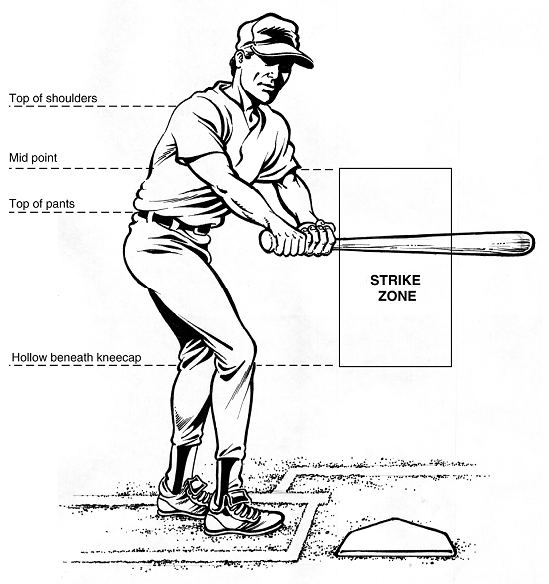
\includegraphics[scale=.3]{Images/strikezone.png}
      	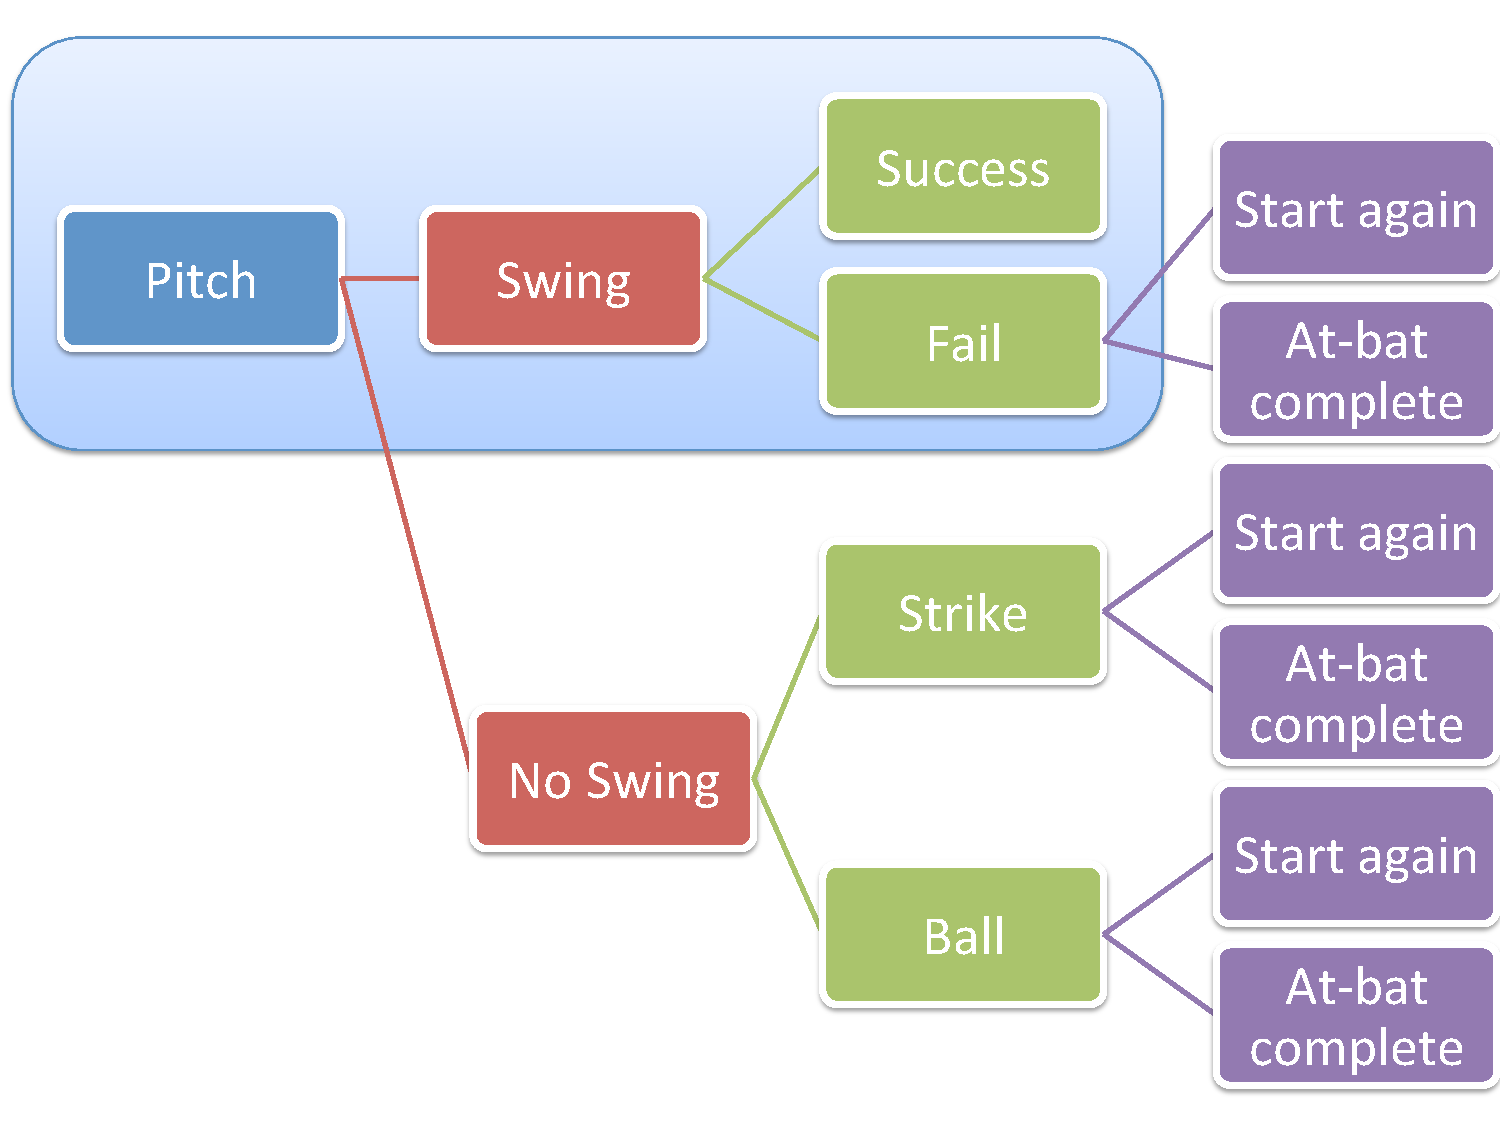
\includegraphics[scale=.3]{Images/HvPTree.pdf}
      	\caption{The image on the left shows the strike zone, from Major League Baseball's rule book. The right-hand image shows an event tree for the hitter vs. pitcher contest in baseball. This paper focuses on the highlighted region. The hitter chooses to swing or not swing at each pitch. If he chooses to swing then, for our purposes, a Bernoulli trial occurs.}
      	\end{figure}
We will call the general airspace over home plate where the hitter swings at the ball the hitting zone. Therefore, the hitting zone includes, but is not limited to, the strike zone. The ``strike zone'' is a plane perpendicular to, and the width of, home plate. It extends from the hitter's knee caps to the midpoint between his belt and shoulders, as shown in Figure 3. 